Besozzi in his PhD thesis (see \cite{Besozzi:PhD:2004}) formulates three criteria that a good P system variant should satisfy:

\begin{enumerate}
	\item It should be as much realistic as possible from the biological point of view, in order not to widen the distance between the inspiring cellular reality and the idealized theory.
	\item It should result in computational completeness and efficiency, which would mean to obtain universal (and hence, programmable) computing devices, with a powerful and useful intrinsic parallelism;
	\item It should present mathematical minimality and elegance, to the aim of proposing an alternative framework for the analysis of computational models.
\end{enumerate}

In membrane computing, many models are equal in power with Turing machines. We should say they are Turing complete (or computationally complete), but because the proofs are always constructive, starting the constructions from these proofs from universal Turing machines or from equivalent devices, we obtain universal P systems (able
to simulate any other P system of the given type). That is why we speak about universality results, and not about computational completeness.

\subsection{Accepting vs generating} % (fold)
\label{sub:accepting_vs_generating}

In the Chomsky hierarchy, there are language acceptors (finite automata, Turing machines) and language generators (formal grammars).

% Accepting grammars

Bordhin in \cite{Bordihn99acceptingpure} extends grammars to allow for accepting languages by interchanging the left side with the right side of a rule. The mode will apply rewriting rules to an input word and accept it when it reaches the starting nonterminal. However, the input word consists of terminal symbols, which could not be rewritten when using original definition, hence they consider the pure version of various grammar types where they give up the distinction between terminal and nonterminal symbols.

% Accepting vs generating common results

The regular, context-free, context-sensitive and recursively enumerable languages were shown to have equal power in accepting and generating mode.
Some other grammars (programmed grammars with appearence checking) are shown to be more powerful in accepting mode than in generating mode.
For deterministic Lindenmeyer systems, the generating and accepting mode are incomparable.

% Accepting vs generating P system results

It can be interesting to investigate accepting and generating mode also in P system variants. Barbuti in \cite{Barbuti:2010:AcceptingGenerating} shown that in the nondeterministic case, when either promoters or cooperative rules are allowed, acceptor P systems have shown to be universal. The same in known to hold for the corresponding classes of nondeterministic generator P systems. In the deterministic case, acceptor P systems have been shown to be universal only if cooperative rules are allowed. Universality has been shown not to hold for the corresponding classes of generator P systems.

% subsection accepting_vs_generating (end)

\subsection{Active vs passive membranes} % (fold)
\label{sub:active_vs_passive_membranes}

% TODO: need citations
Most of the studied P system variants assumes that the number of membranes can only decrease during a computation, by dissolving membranes as a result of applying evolution rules to the objects present in the system.
A natural possibility is to let the number of membranes also to increase during a computation, for instance, by division, as it is well-known in biology. Actually, the membranes from biochemistry are not at all passive, like those in the models briefly described above.
For example, the passing of a chemical compound through a membrane is often done by a direct interaction with the membrane itself (with the so-called protein channels or protein gates present in the membrane); during this interaction, the chemical compound which passes through membrane can be modified, while the membrane itself can in this way be modified (at least locally).

In \cite{Paun99ActiveMembranes} Paun considers P systems with active membranes where the central role in the computation is played by the membranes: evolution rules are associated both with objects and membranes, while the communication through membranes is performed with the direct participation of the membranes; moreover, the membranes can not only be dissolved, but they also can multiply by division. An elementary membrane can be divided by means of an interaction with an object from that membrane.

% Polarisation

Each membrane is supposed to have an electrical polarization (we will say charge), one of the three possible: positive, negative, or neutral. If in a membrane we have two immediately lower membranes of opposite polarizations, one positive and one negative, then that membrane can also divide in such a way that the two membranes of opposite charge are separated; all membranes of neutral charge and all objects are duplicated and a copy of each of them is introduced in each of the two new membranes.
The skin is never divided.
If at the same time a membrane is divided and there are objects in this membrane which are being rewritten in the same step, then in the new copies of the membrane the result of the evolution is included.

In this way, the number of membranes can grow, even exponentially. As expected, by making use of this increased parallelism we can compute faster.
For example, the SAT problem, which is NP complete, can be solved in linear time, when we consider the steps of computation as the time units.
Moreover, the model is shown to be computationally universal.

% subsection active_vs_passive_membranes (end)

\subsection{Context in rules} % (fold)
\label{sub:context_in_rules}

% Cooperative / Non-cooperative

Rewriting rules in P systems can be cooperative and non-cooperative, like in Chomsky's context-free and context-sensitive grammars. Non-cooperative rules are restricted to use only one object on the left side and cooperative rules do not have this restriction.
P systems with cooperative rules are universal \cite{Paun98}, while P systems with non-cooperative rules only characterize parikh image of context-free languages ($PsCF$) \cite{Sburlan05dragos}.

% Catalytic P systems

Paun \cite{Paun98} also defines P systems with catalysts where catalysts are a specified subset of the alphabet. Rewriting rules can contain catalysts, which are not modified by applying the rule. Suprisingly, P systems with catalytic rules are universal, actually two membranes in the P system are sufficient to achieve universality.

In systems with only catalytic rules (purely catalytic systems), three catalysts are enough. <citation needed> % TODO: need cite

% Two catalysts

Freund in \cite{Freund2005TwoCatalysts} shows that two catalysts are enough and raised an open problem whether one catalyst is sufficient. He conjectured that for computationally universal P systems the results obtained in this paper are optimal not only with respect to the number of membranes (2), but also with respect to the number of catalysts.

% Catalysts are too powerful

From some point of view, catalysts are way too powerful in restricting the parallelism - they directly participate in the rules, hence the number of catalytic rules that can be applied in one step, is bounded by number of catalysts.

A variant with promoters and inhibotors have been proposed (see \cite{Ionescu:jucs_10_5:on_p_systems_with}).

% Promoters

In the case of promoters, the rules are possible only in the presence of certain symbols. An object $p$ is a promoter for a rule $u\rightarrow v$ and we denote this by $u\rightarrow v|_{p}$, if the rule is active only in the presence of object $p$. Note that unlike in the case with catalysts, promoters allow the associated rules to be applied as many times as possible.

% Inhibitors

An object $i$ is inhibitor for a rule $u\rightarrow v$ and we denote this by $u\rightarrow v|_{\neg i}$, if the rule is active only if inhibitor $i$ is not present in the region.

% TODO: add reference

One of our results uses inhibitors as a tool to achieve universality for sequential P systems.


% One catalyst with promoters/inhibitors

Ionescu in \cite{Ionescu:jucs_10_5:on_p_systems_with} shows that P systems with non-cooperative catalytic rules with only one catalyst and with promoters/inhibitors are universal.

% Zero catalysts with inhibitors

Non-cooperative rules with no catalysts and with inhibitors were studied in \cite{Sburlan:2006:FurtherResultsPromotersInhibitors}, the equivalence with Lindenmeyer systems ($ET0L$ as defined in section \ref{sec:lindenmeyer_systems}) was proved.

% Simple cooperative system

Dang \cite{Ibarra04dang} proposes a simple cooperative system ($SCO$) as a P system where the only rules allowed are of the form $a\rightarrow v$ or of the form $aa\rightarrow v$, where $a$ is a symbol and $v$ is a (possibly null) string of symbols not containing $a$. This variant is investigated with various modes of parallelism, so their results will be mentioned in the subsection \ref{sub:parallelism_options}

% subsection context_in_rules (end)

\subsection{Rules with priorities} % (fold)
\label{sub:rules_with_priorities}

In the original definition of a P system \cite{Paun98}, a partial order relation over set of rewriting rules have been specified. The rule can be used only if no rule of a higher priority in the region can be applied at the same time.

Sos\'ik in \cite{Sosik:2002:WithoutPriorities} showed that the priorities may be omitted from the model without loss of computational power.

% subsection rules_with_priorities (end)

\subsection{Energy in P systems} % (fold)
\label{sub:energy_in_p_systems}

Various notions of energy has been proposed for use in P systems. Paun in \cite{Paun:2001:Energy} considers a P system where each evolution rule ``produces'' or ``consumes'' some quantity of energy, in amounts which are expressed as integer numbers. In each moment and in each membrane the total energy involved in an evolution step should be positive, but if ``Soo much'' energy is present in a membrane, then the membrane will be destroyed (dissolved). This variant was investigated in two cases, both were shown to be universal:

\begin{enumerate}
	\item when using only two membranes and unbounded amount of energy,
	\item when using arbitrarily many membranes and a bounded energy associated with rules
\end{enumerate}

Freund in \cite{Freund:2004:SequentialEnergy} introduced a new variant where the rules are assigned directly to membranes (every rule consume objects on one side of the membrane and produce objects on the other side) and every membrane carries an energy value that can be changed during a computation by objects passing through the membrane.

This variant is universal even in sequential mode if we allow priorities on the objects. When omitting the priority relation, only the family of Parikh sets generated by context-free matrix grammars ($PsMAT$ as defined in section \ref{sec:matrix_grammars}) is obtained.

% subsection energy_in_p_systems (end)

\subsection{Symport/antiport rules} % (fold)
\label{sub:symport_antiport_rules}

Paun in \cite{Paun:2002:SymportAntiport} proposes a new way of communicating between membranes.

Symports allow two chemicals to pass together through a membrane in the same direction using symport rules of type $(ab,in)$ or $(ab,out)$.
Antiports allow two chemicals to pass simultaneously through a membrane in opposite directions using antiport rules of type $(a,in;b,out)$.

Suprisingly, a P system variant, where only the symport/antiport rules are used are computationally complete. Five membranes are enough for this result. If more than two chemicals may collaborate when passing through membranes, two membranes are sufficient for universality. These results are proven in \cite{Paun:2002:SymportAntiport}.

% subsection symport_antiport_rules (end)

\subsection{Parallelism options} % (fold)
\label{sub:parallelism_options}

Original definition of P system (see \cite{Paun98}) uses maximal parallelism when doing a step of computation. There is an obvious biological motivation relying on the assumption that ``if we wait long enough, then all reaction which may take place will take place''. This condition is rather powerful, because it decreases the non-determinism of the sysem's evolution. For various reasons ranging from looking for more realistic models to just the mathematical challenge, the maximal parallelism was questioned.

% Sequential mode

Dang in \cite{Dang04Sequential} investigates the sequential mode. In each step, from the set of applicable rules across all membrane one is nondeterministically chosen and applied. For purely catalytic systems with 1 membrane, the sequential mode generates only the semilinear sets and thus is strictly weaker than the maximally parallel version.
% TODO: add semilinear sets
Sequential version of symport/antiport systems are equivalent to vector addition systems making it strictly weaker than the original maximally parallel version.

Investigation of the sequential mode continues in \cite{Dang:2005:Sequential}. Sequential P system without priorities with cooperative rules with rules for membrane dissolution are not universal by showing they can be simulated by vector addition systems with states (VASS).
This holds even when the membrane creation is allowed for bounded number of created membranes. However, if any number of membranes are allowed to be created, the system becomes universal. This result was shown by simulation of the register machine (see section \ref{sec:register_machines}).

%TODO: add reference

We have further investigated this variant (sequential P system without priorities with cooperative rules) by allowing rules with inhibitors, which resulted in universality.


% Restricting maximal parallelism

Dang in \cite{Ibarra04dang} proposes several restricted versions of parallelism.
$n${\bf -Max-Parallel} version nondeterministically selects a maximal subset of at most n rules to apply. It is proved that 9{\bf -Max-Parallel} SCO (defined in the subsection \ref{sub:context_in_rules}) is universal.
$\leq n${\bf -Parallel} version is similar, but does not require the condition of a maximal subset of rules. It is shown to be weaker than $n${\bf -Max-Parallel} version.
$n${\bf -Parallel} version requires the size of the subset of rules to apply to be exactly $n$.
All three versions are equal to the sequential mode when $n=1$. For non-universality results, Dang used the proof technique by simulation by vector addition systems. Our future research may be inspired by this techniue.

% Minimal parallelism

Ciobanu in \cite{Ciobanu:2007:MinimalParallelism} proposes a minimal parallelism: for each region if at least one rule can be applied, then at least one rule will be applied. The symport/antiport rules variant and variant with active membranes were both shown to be universal.

% Asynchronous

Freund in \cite{Freund:2004:Async} studied the asynchronous mode of P systems, where in each step, arbitrary many rules can be applied. The application of rules is hence done in parallel way, but are not synchronized or somewhat controlled. In many cases the sequential and asynchronous modes were shown to be equivalent.

% subsection parallelism_options (end)

\subsection{Sequential P systems without priorities with cooperative rules and inhibitors} % (fold)
\label{sub:sequential_p_systems_without_priorities_with_cooperative_rules_and_inhibitors}

Original definition of P systems with inhibitors (see \cite{Ionescu:jucs_10_5:on_p_systems_with}) allow to use only one inhibitor pre rule, e.g. $u\rightarrow v|_{\neg i}$. Alternative definition (see \cite{Agrigoroaiei:2010:Dissolution}) allow to use whole inhibitor set in the rule like $u\rightarrow v|_{\neg B}$, where $B$ is a set of objects. Such a rule can be applied only if no element of $B$ is present in the region.

For sequential P systems, the following lemma will show the equivalence of these definitions. However, special condition must be fulfilled, the regions with such rules cannot be empty.

% !TEX root = ../diz.tex
\begin{lemma}
\label{lemma:inhibitor_step}
  If there is at least one object present in each region of a P system, rewriting step in P system with inhibitor set can be simulated by multiple consecutive steps of P system with single inhibitor.
\end{lemma}

\begin{dokaz}
  Consider a P system with the alphabet $\Sigma$.
  For each rule $u\rightarrow v|_{\neg B}$, where $B=\{b_1, b_2, \dots ,b_n\}$ we will have rules:
    \begin{align*}
      c\rightarrow&c|GONE_{b}|_{\neg b} \text{~for all~} c\in \Sigma, b\in B \\
      u|GONE_{b_1}|GONE_{b_2}|\dots|GONE_{b_n}\rightarrow&v|GONE_{b_1}|GONE_{b_2}|\dots|GONE_{b_n}
    \end{align*}

\end{dokaz}

Note that symbols $GONE_b$ are created automatically when some object $c$ is present in the region. 

\begin{veta}
  The sequential P system with inhibitors defines the same Parikh image of language as P system with maximal parallelism.
\end{veta}

\begin{dokaz}
  We show that we can simulate maximal parallel step of P system with several steps of sequential P system with inhibitors. The proof is quite technical with some workarounds.

  % Membrane states

  It is important to note that in the maximal parallel step the rewriting occurs in all membranes, so we need to synchronize this process. Every membrane will have a state, represented as an object.

  The $RUN$ state represents that the rewriting still occurs. When there are no more rules to apply, the region has done its maximal parallel step and proceeds to the state $SYNCHRONIZE$. Other states are just technical - we need to implement sending objects between membranes and preparing for the next maximal parallel step by unmarking newly created objects in the current maximal parallel step, which have been marked to prevent double rewriting in one step.

  \begin{itemize}
    \item $RUN$: Rewriting occurs. Objects that are to be sent to the parent membrane are directly sent because the parent membrane is already in $RUN$ or $SYNCHRONIZE$ phase, so the $a^{\prime}$ symbols that are sent don't break anything. But objects that are to be sent down, cannot be sent immediately because child membranes can be in the previous phase waiting to restore symbols from previous step. Current symbols could interfere with them and be rewritten twice in this step. Such objects are only marked as ``to be sent down'': $a^{\downarrow\prime}$

    \item $SYNCHRONIZE$: Rewriting has ended and the membrane is waiting to get signal $SYNCED$ from the parent membrane to continue to the next step.

    \item $SENDDOWN$: Signal $SYNCED$ was caught and now all descendant membranes are in $SYNCHRONIZE$ phase so $a^{\downarrow\prime}$ can be sent down.

    \item $RESTORE$: All $a^{\prime}$ symbols are being restored to $a$, so the next step of rewriting can take place.
  \end{itemize}

  % Rewriting rules

  \begin{itemize}
    \item For every rule $r_i\in R$ such that
      \begin{align*}
        r_i = a_1^{M(a_1)}a_2^{M(a_2)}\dots a_n^{M(a_n)} \rightarrow a_1^{N(a_1)}a_2^{N(a_2)}\dots a_n^{N(a_n)}
      \end{align*}
      we will have the following rules:
      \begin{align*}
        &a_1^{M(a_1)-m_1}\dot{a}_1^{m_1}
        a_2^{M(a_2)-m_2}\dot{a}_2^{m_2}\dots
        a_n^{M(a_n)-m_n}\dot{a}_n^{m_n}|RUN \\
        \rightarrow &a_1^{\prime N(a_1)}a_2^{\prime N(a_2)}\dots a_n^{\prime N(a_n)}|RUN
      \end{align*}
      
      There will be such rule for each $0\leq m_i\leq M(a_i)$. It represents the idea that $\dot{a}$ can be used in rewriting in the same way as $a$. Right side of the rules contains symbols $a^\prime$, that prevents the symbols to be rewritten again.

    \item For every symbol $a\in V$ we will have the following rules:

    $a|RUN \rightarrow \dot{a}|RUN|_{\neg \dot{a}}$

    There will be at most one occurrence of $\dot{a}$.

    \item For every rule $r_i\in R$ there will be a rule that detects if the rule $r_i$ is not applicable. According to left side of the rule $r_i$, symbol $UNUSABLE_i$ will be created when there is not enough objects to fire the rule $r_i$. It means that left side of rule $r_i$ requires more instances of some object than are present in membrane.

    If the left side is of type:
    \begin{itemize}
      \item $a$: It is a context free rule. The rule can't be used if there is no occurrence of $a$ nor $\dot{a}$.

      $RUN \rightarrow UNUSABLE_i|RUN|_{\neg\{UNUSABLE_i, a, \dot{a}\}}$

      \item $ab$: It is a cooperative rule with two distinct objects on the left side. The rule cannot be used if there is one of them missing.

      $RUN \rightarrow UNUSABLE_i|RUN|_{\neg\{UNUSABLE_i, a, \dot{a}\}}$

      $RUN \rightarrow UNUSABLE_i|RUN|_{\neg\{UNUSABLE_i, b, \dot{b}\}}$

      \item $a^2$: It is a cooperative rule with two same objects. The rule can't be used if there is at most one occurrence of the symbol. That happens if there is no occurrence of $a$. There can still be $\dot{a}$, but at most one occurrence.

      $RUN \rightarrow UNUSABLE_i|RUN|_{\neg\{UNUSABLE_i, a\}}$
    \end{itemize}

    \item For every membrane with label $i$ there will be a rule:
    \begin{align*}
      &UNUSABLE_1|UNUSABLE_2|\dots|UNUSABLE_m|RUN \\
      \rightarrow &SYNCHRONIZE|SYNCTOKEN_i\uparrow
    \end{align*}

    If no rule can be used, maximal parallel step in the region is completed hence it goes to the synchronization phase and sends a synchronization token to the parent membrane.

    \item For every membrane there will be a rule:
    \begin{align*}
      &SYNCHRONIZE|SYNCTOKEN_j \\
      \rightarrow &SYNCHRONIZE|SYNCTOKEN_j\uparrow
    \end{align*}

    Membrane resends all synchronization tokens from child membranes to the parent membrane.

    \item In the skin membrane there is a rule which collects all the synchronization tokens from all membranes $1\dots k$ and then sends down signal that synchronization is complete. But before that, there can be some symbols that should be sent down, but they weren't, because the region below could have not started the rewriting phase that time. The result was just marked with $a^{\downarrow\prime}$.
    \begin{align*}
      &SYNCTOKEN_1|\dots|SYNCTOKEN_k|SYNCHRONIZE \\
      \rightarrow &SENDDOWN
    \end{align*}

    \item Every membrane other than skin membrane have to receive the signal to go to the senddown phase:

    $SYNCHRONIZE|SYNCED \rightarrow SENDDOWN$

    \item Every membrane will have rules for every symbol $a\in V$ to send down all unsent objects that should have been sent down:

    $SENDDOWN|a^{\downarrow\prime} \rightarrow SENDDOWN|a^{\prime}\downarrow$

    \item Every membrane will have a rule for detecting when all such objects have been sent and it goes to restore phase:

    $SENDDOWN \rightarrow RESTORE|_{\neg \{a_i^{\downarrow\prime}|1\leq i\leq n\}}$

    \item In the restore phase all symbols $a^{\prime}$ will be rewritten to $a$ in order to be able to be rewritten in the next maximal parallel step:

    $RESTORE|a^{\prime} \rightarrow RESTORE|a$
    
    \item When using lemma~\ref{lemma:inhibitor_step}, there may be some $GONE$ symbols left and now is the time to clear them:

    $RESTORE|GONE_i \rightarrow RESTORE$

    \item When the restore phase ends, it sends down a signal that all membranes have been already synchronized and next phase of rewriting has began in upper membranes:

    $RESTORE \rightarrow RUN|SYNCED\downarrow|_{\neg \{a_i^{\prime}|1\leq i\leq n\}\cup\{GONE_i|1\leq i\leq n\}}$
  \end{itemize}

  \definecolor{run}{rgb}{1,0.5,0}
  \definecolor{restore}{rgb}{0,0.5,0}
  \definecolor{synchronize}{rgb}{0,0,1}
  \definecolor{senddown}{rgb}{1,0,0}
  % Narrow texts in boxes
  \providecommand{\narrow}[1]{\scalebox{.85}[1.0]{#1}}

  \begin{figure}
    \def\svgwidth{\textwidth}
    \input{possible_pairs_of_states_of_parent_and_child_membrane.pdf_tex}
    % 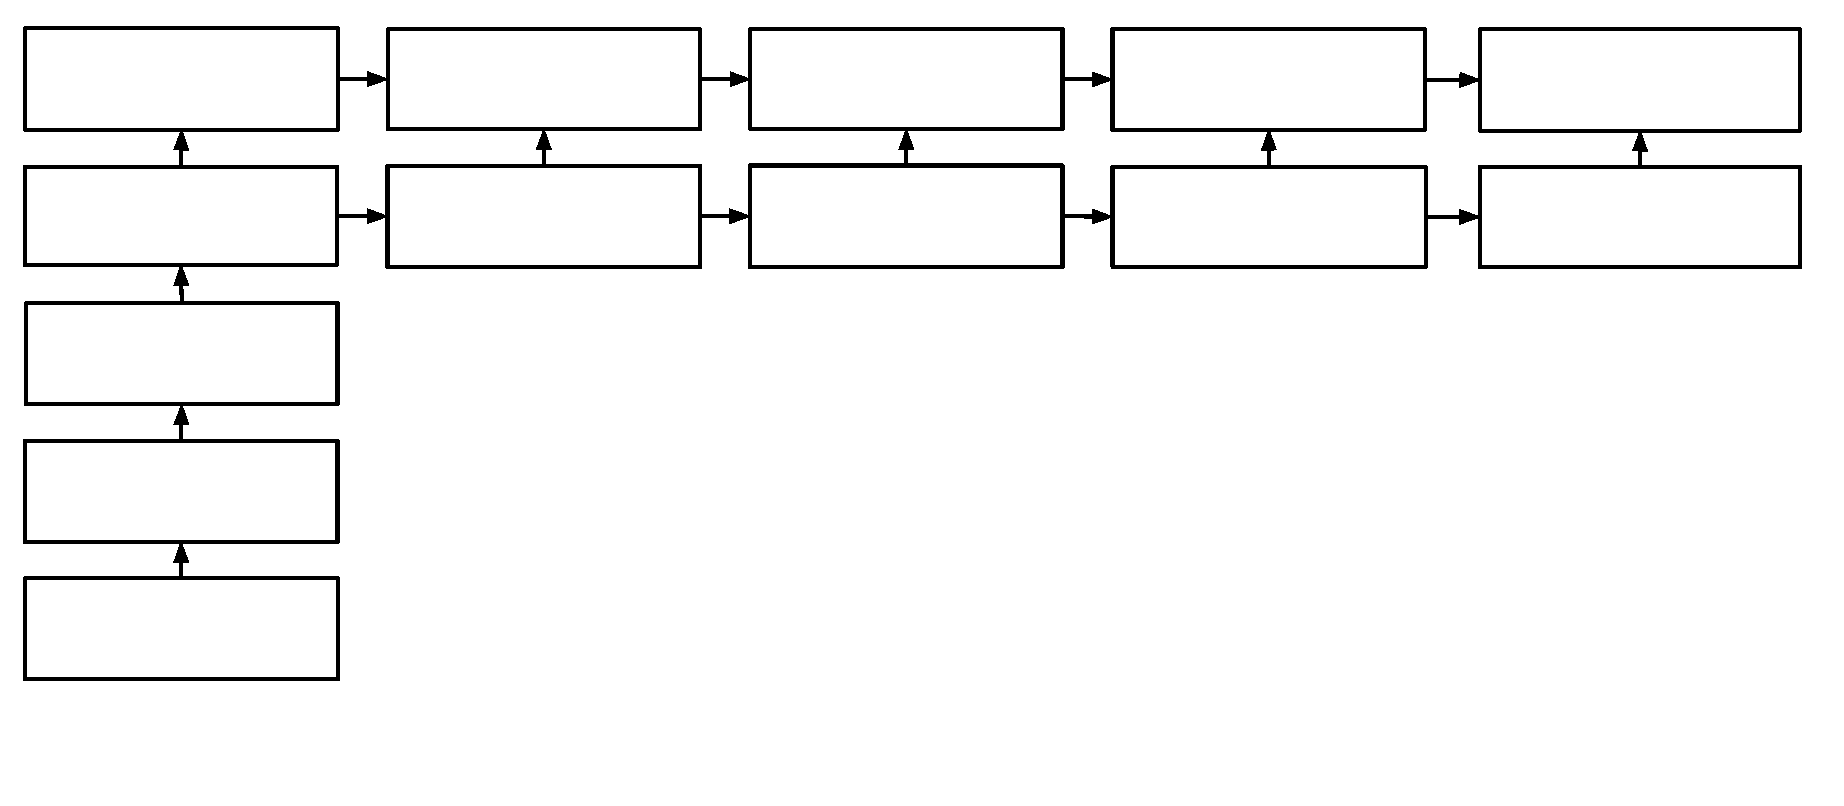
\includegraphics[width=\textwidth]{possible_pairs_of_states_of_parent_and_child_membrane}
    \caption{Possible pairs of states of parent and child membrane}
    \label{fig:possible_pairs_of_states_of_parent_and_child_membrane}
  \end{figure}

  \begin{figure}
    \def\svgwidth{\textwidth}
    \input{snapshot_of_all_membrane_states_while_simulating.pdf_tex}
    % 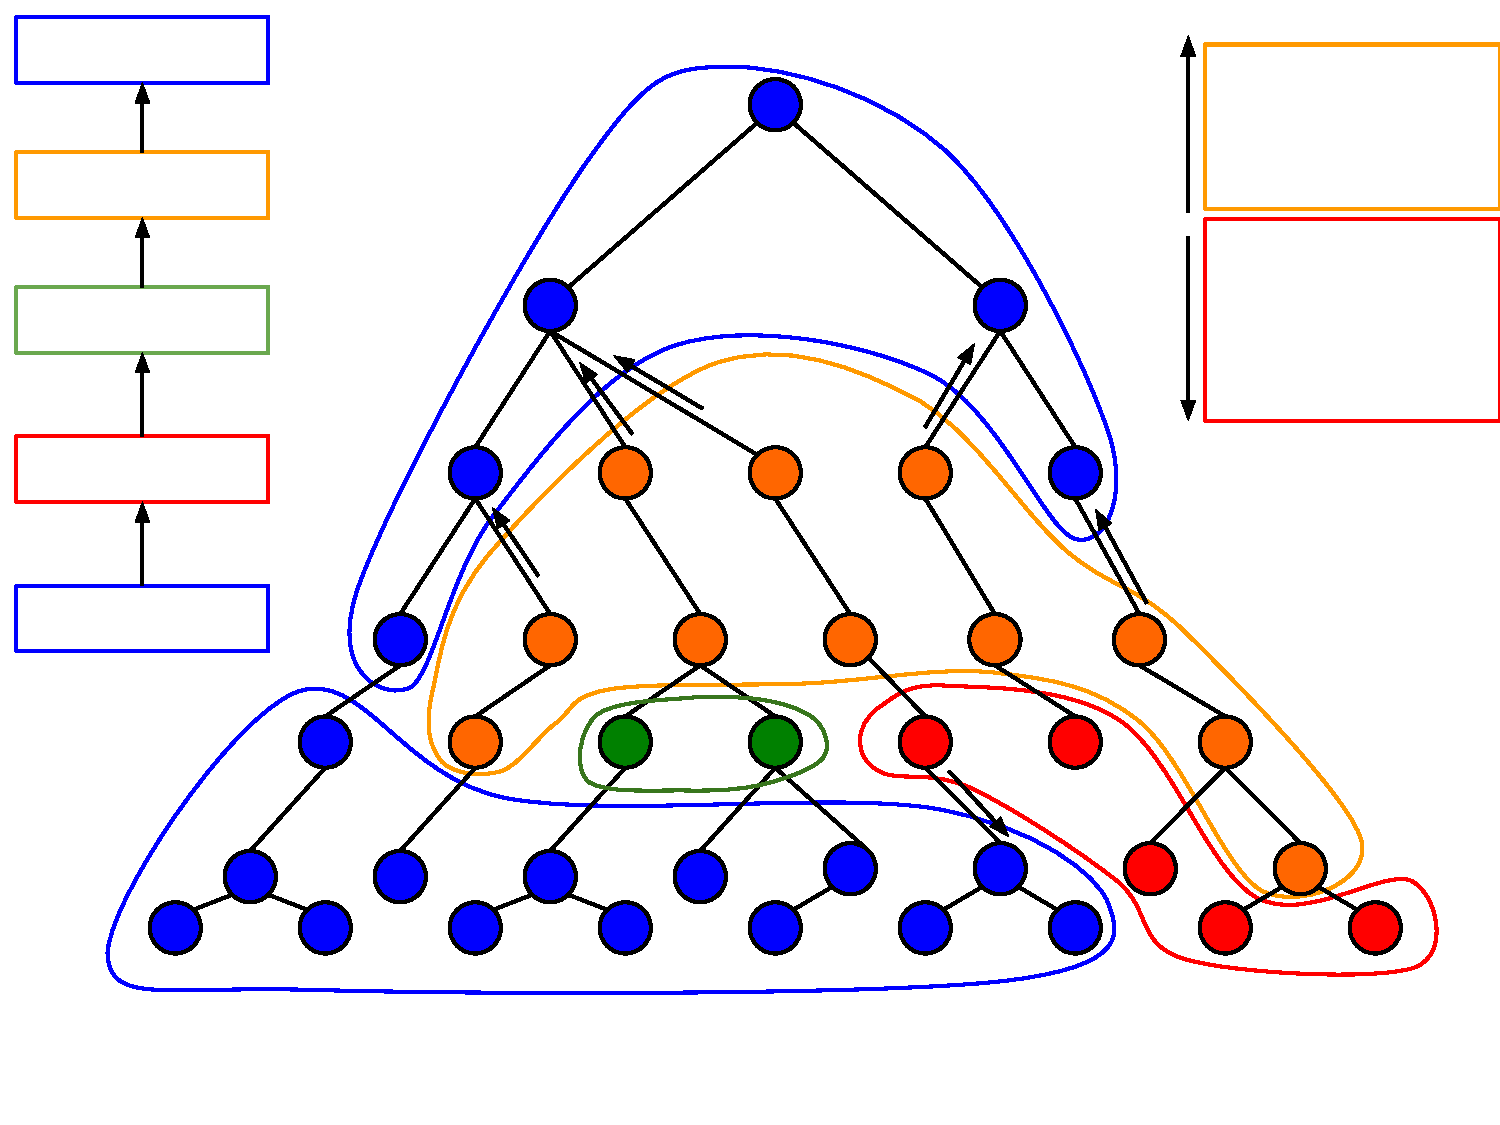
\includegraphics[width=\textwidth]{snapshot_of_all_membrane_states_while_simulating}
    \caption{Snapshot of all membrane states while simulating}
    \label{fig:snapshot_of_all_membrane_states_while_simulating}
  \end{figure}

  The pairs of possible phases of the parent and child membrane are shown in the figure \ref{fig:possible_pairs_of_states_of_parent_and_child_membrane} along with transitions between two consecutive global synchronizations - after the maximal parallel steps $i$ and $i+1$.

  In the figure \ref{fig:snapshot_of_all_membrane_states_while_simulating} the membrane structure is presented as a hierarchical structure. Every membrane is in one of four phases. It can be seen that the sending of the objects is performed in such phases that the receiving membrane is in either $RUN$ or $SYNCHRONIZE$ phase, so the received objects (marked $a^\prime$) does not interfere with rewriting.

  Another interesting idea can be seen in the figure \ref{fig:snapshot_of_all_membrane_states_while_simulating} that when a region is in the $SENDDOWN$ phase and objects are sent through the child membrane, the receiving region is in the $SYNCHRONIZE$ phase waiting for the $SYNCED$ signal, which will be sent to it when $SENDDOWN$ and $RESTORE$ phases finished.

  All membranes are nonempty during the simulation because at least the object representing the current phase is always present. By lemma~\ref{lemma:inhibitor_step} the rules with set of inhibitors can be simulated by single inhibitors.


\end{dokaz}




We have also reached this result in the accepting case by simulation of register machines.

\begin{veta}
  Sequential P systems with inhibitors can simulate register machines and thus equal $PsRE$.
\end{veta}


\begin{dokaz}
\label{proof:reg_by_inh}
  Suppose we have a $n$-register machine $M = (n,P,i,h)$. In our simulation we will have a membrane structure consisting of one membrane and the contents of register $j$ will be represented by the multiplicity of the object $a_j$.

  We will have P system $(V, \mu, w, R)$, where:
  \begin{itemize}
    \item $V$ is an alphabet consisting of symbols that represent registers $a_1,\dots a_n$ and instruction labels in $Lab(M)$,
    \item $\mu$ is a membrane structure consisting of only one membrane,
    \item $w$ is initial contents of the membrane. It contains symbols for the input for the machine $a_i^{n_i}$ where $n_i$ is initial state of register with label $i$ and initial instruction $e \in Lab(M)$.
    \item $R$ is the set of rules in the skin membrane:
    
    For all instructions of type $(e : add(j), f)$ we will have rule:
    \begin{itemize}
      \item $e \rightarrow a_j|f$.
    \end{itemize}
    
    For all instructions of type $(e : sub(j), f, z)$ we will have rules:
    \begin{itemize}
      \item $e|a_j \rightarrow f$ and
      \item $e \rightarrow z|_{\neg a_j}$.
    \end{itemize}

    And finally halting rules:
    \begin{itemize}
      \item $h|a_j \rightarrow h|\#$ for all $a\leq j\leq n$,
      \item $\# \rightarrow \#$,
    \end{itemize}
  \end{itemize}

  When the halting instruction is reached, if there is an object present in the membrane, the hash symbol $\#$ is created and it will cycle forever. If there is no object present, there is no rule to apply and computation will halt. It corresponds to the condition that all registers should be empty when halting.
\end{dokaz}

% subsection sequential_p_systems_without_priorities_with_cooperative_rules_and_inhibitors (end)

\subsection{Vacuum} % (fold)
\label{sub:vacuum}

We propose a new variant of P system with vacuum. In the common sense, vacuum represents a state of space with no or a little matter in it. Using vacuum in modelling frameworks can help express certain phenomena more easily. We define a new P system variant, which creates a special vacuum object in a region as soon as the region becomes empty. The vacuum is removed whenever some object interacts with it. After the interaction, there is vacuum no longer. This removal process is realized by allowing the vacuum object to be used only on the left side of rules. If we made the vacuum to be removed automatically when an object enters the region, there would be no difference with the variant without vacuum objects because of no interactions with it.
We are interested in how the variant with the vacuum improves the computation power of a sequential P system in comparison to the variant without using the vacuum.

\begin{veta}
  The sequential P system with Vacuum is universal.
\end{veta}

\begin{dokaz}
  We can simulate the variant of P system where the only cooperative rule is of type $a|a \rightarrow b$. According to \cite{Ibarra04dang} the variant, where the only cooperative rule is when both objects are the same, is universal. If there is no rule $a \rightarrow b$, we can rewrite $a$ to $a^{\prime}$ so we can mark all present symbols. $a^{\prime}$ symbols are kept in special membrane so the Vacuum can be created in main membrane and we can synchronize.
  
  But we won't do this madness again.
  
  Instead, we will try to prove universality by simulating the register machine. We need to detect when the current register is empty. If there was a symbol for every register as in the proof~\ref{proof:reg_by_inh}, the Vacuum would be created only if all registers are empty. But the $sub()$ instruction need to detect when one concrete register is empty.
  
  We will have a membrane for each register. That membrane will be contained in the skin membrane. The number of objects in membrane $i$ will correspond to the value of register $i$.
  
  The alphabet will consist of instruction labels and register counter $a$. The skin membrane will only have an instruction label. It is sent to corresponding membrane where the instruction is executed. Then, the following instruction is sent back to the skin membrane.
  
  We will have following rules in the skin membrane:
  
  \begin{itemize}
  \item $e \rightarrow e\downarrow_j$ for an instruction of type $e : add(j), f$ or $e : sub(j), f, z$ and
  \item $h \rightarrow h\downarrow$ for a halting instruction h.
  \end{itemize}
  
  And in non-skin membranes:
  
  \begin{itemize}
  \item $e \rightarrow a|f\uparrow$ instructions of type $e : add(j), f$,
  \item $e|a \rightarrow f\uparrow$ for instructions of type $e : sub(j), f, z$,
  \item $e|VACUUM \rightarrow z\uparrow$ for instructions of type $e : sub(j), f, z$, and
  \item $h|a \rightarrow h|a$
  \end{itemize}

  When halting, if there is an nonempty register, it will cycle forever with the last rule. However, if all registers are empty, the halting instruction label will stay in all membranes and the computation will halt.
  
\end{dokaz}

% subsection vacuum (end)